\documentclass{article}
\usepackage[T1]{fontenc}
\usepackage{graphicx}
\usepackage{amsmath, amsthm, amssymb}
\usepackage{hyperref}
\usepackage{polski}
\usepackage{listings}
\usepackage{enumerate}
\newtheorem{theorem}{Twierdzenie}
\theoremstyle{definition}

\newtheorem{definition}{Definicja}

\title{Tytuł}
\author{Zuzanna Pawlik}
\date{\today}
\begin{document}

\maketitle
\section*{Obraz z pliku pdf}
\begin{center}
	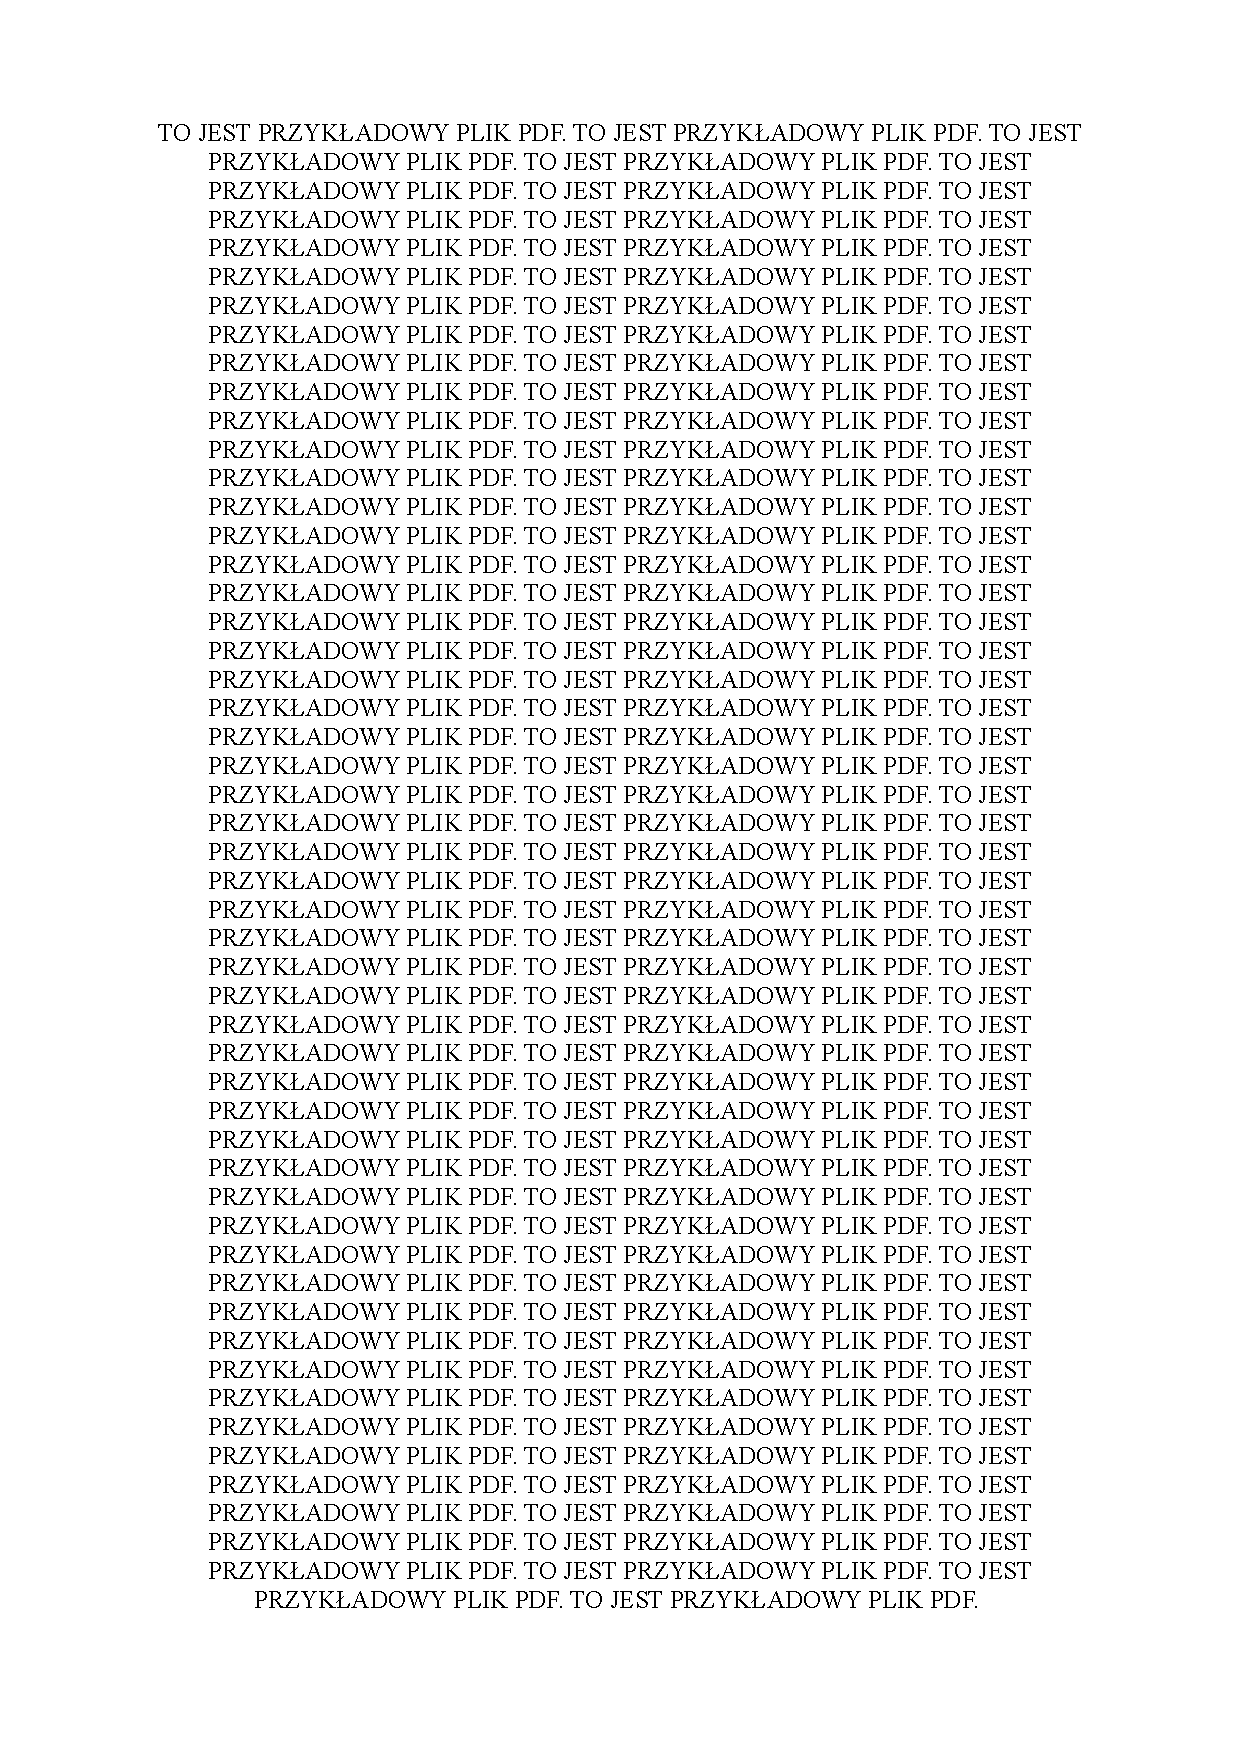
\includegraphics[height=5cm]{obraz1.pdf}
\end{center}


\section*{Wyliczenia}
\subsection*{litery}
\begin{enumerate}[a)]
	\item punkt a
	\item punkt b
	\item punkt c
\end{enumerate}

\subsection*{liczby}
\begin{enumerate}
	\item punkt 1
	\item punkt 2
	\item punkt 3
\end{enumerate}

\subsection*{punkty}
\begin{itemize}
	\item pierwszy
	\item drugi
	\item trzeci
\end{itemize}

\section*{Wzory matematyczne}
\subsection*{w tekście}
to jest tekst ze wzorem $c^2 = a^2 + b^2$ w środku

\subsection*{wyróżnione}
Tutaj mamy wyróznione wzory

\[f(x) = ax^2 + bx + c\]
\[\Delta = b^2 - 4ac\]
\[x_{1} = \frac{-b + \sqrt{\Delta}}{2a}\]
\[x_{2} = \frac{-b - \sqrt{\Delta}}{2a}\]

\subsection*{numerowane}
\begin{equation}
	\lim\limits_{x \to 0}\frac{sin(x)}{x} = 1
\end{equation}

\section*{Tabela}
\begin{table}[h]
\centering
\begin{tabular}{|c|c|c|}
\hline
 & kolumna1 & kolumna2\\
\hline
wiersz1 & 1 & 2\\
\hline
wiersz2 & 2 & 4\\
\hline
\end{tabular}
\end{table}

\begin{thebibliography}{2}
\bibitem{citekey}Imie Nazwisko \emph{Tytuł, z podtytułem i jeszcze trochę}, Miejsce, 30.02.1999
\bibitem{citekey}Ktoś Inny \emph{I jego książka też jest cytowana}, Miasto, 12.34.5678
\end{thebibliography}



\end{document}